% Created 2020-02-11 Tue 18:45
% Intended LaTeX compiler: pdflatex
\documentclass[presentation,aspectratio=169,smaller]{beamer}
\usepackage[utf8x]{inputenc}
\usepackage[T1]{fontenc}
\usepackage{graphicx}
\usepackage{grffile}
\usepackage{longtable}
\usepackage{wrapfig}
\usepackage{rotating}
\usepackage[normalem]{ulem}
\usepackage{amsmath}
\usepackage{textcomp}
\usepackage{amssymb}
\usepackage{capt-of}
\usepackage{hyperref}
\usepackage{color}
\usepackage[newfloat]{minted}
\usepackage[utf8]{inputenc}
\usepackage{soul}
\usepackage{unicode-math}
\usepackage{mathtools}
\usepackage[mathletters]{ucs}
\usemintedstyle{tango}
\setminted{fontsize=\scriptsize}
\setminted{mathescape=true}
\setbeamertemplate{itemize items}[circle]
\setbeamertemplate{enumerate items}[default]
\setlength{\parskip}{\baselineskip}%
\setlength{\parindent}{0pt}%
\setbeamertemplate{navigation symbols}{}%remove navigation symbols
\newcommand{\hlyellow}[1]{\colorbox{yellow!50}{$\displaystyle#1$}}
\newcommand{\hlfancy}[2]{\sethlcolor{#1}\hl{#2}}
\usetheme{default}
\author{Boris Buliga}
\date{\today}
\title{Universe of zippers (or how to plant a bomb)}
\hypersetup{
 pdfauthor={Boris Buliga},
 pdftitle={Universe of zippers (or how to plant a bomb)},
 pdfkeywords={},
 pdfsubject={},
 pdfcreator={Emacs 28.0.50 (Org mode 9.3.1)}, 
 pdflang={English}}
\begin{document}

\maketitle
\newcommand{\mathcolorbox}[2]{%
  \begingroup
  \setlength{\fboxsep}{2pt}%
  \colorbox{#1}{$\displaystyle #2$}%
  \endgroup
}

\AtBeginSection[]{
  \begin{frame}
  \vfill
  \centering
  \begin{beamercolorbox}[sep=8pt,center,shadow=true,rounded=true]{title}
    \usebeamerfont{title}\insertsectionhead\par%
  \end{beamercolorbox}
  \vfill
  \end{frame}
}

\section*{Intro}
\label{sec:orge5ef74d}
\begin{frame}[label={sec:org0e65d48}]{About me}
\begin{columns}
\begin{column}{0.75\columnwidth}
\begin{itemize}
\item Server developer @Wix.
\item Haskell ↔ Emacs Lisp extremist. Whatever that means.
\item Chinese tea lover.
\item Wine-lifestyle activist (92\% of my life).
\end{itemize}
\end{column}

\begin{column}{0.25\columnwidth}
\begin{center}
\includegraphics[height=3.5cm]{images/boris.jpg}
\end{center}
\end{column}
\end{columns}
\end{frame}

\begin{frame}[label={sec:org0580b4a}]{Agenda}
\begin{itemize}
\item <1-> Elementary Cellular Automata
\item <2-> Conway's Game of Life
\item <3-> Bomberman
\end{itemize}
\end{frame}

\section{Act 1: Elementary Cellular Automata}
\label{sec:orgbf461cc}

\begin{frame}[label={sec:org9bb2f6c}]{Cellular Automaton}
A cellular automaton is a collection of "colored" \alert{cells} on a \alert{grid} of
specified shape that evolves through a number of discrete time \alert{steps} according
to a set of \alert{rules} based on the states of neighboring cells.

The rules are then applied \emph{iteratively} for as many time steps as desired.
\end{frame}

\begin{frame}[label={sec:orged2972e}]{Many grids}
\begin{enumerate}
\item one-dimensional line;
\item rectangle grid;
\item square grid;
\item triangular grid;
\item hexagonal grid;
\item d-dimensional integer lattice.
\end{enumerate}
\end{frame}

\begin{frame}[label={sec:org87a9011},t]{Elementary Cellular Automata}
\begin{onlyenv}<1->
Each cell has a value \(a \in \lbrace 0, 1 \rbrace = \lbrace \square, \blacksquare
\rbrace\)
\end{onlyenv}

\begin{onlyenv}<2->
Grid is endless one-dimensional strip/line.
\end{onlyenv}

\begin{onlyenv}<3->
\begin{equation*}
\dots
\square \blacksquare \blacksquare \square \square \square \blacksquare
\dots
\end{equation*}
\end{onlyenv}

\begin{onlyenv}<4->
Next value of the cell is based on it's current value and the values of it's two
neighbours (left and right).

\begin{equation*}
  r : (a, a, a) \rightarrow a
\end{equation*}
\end{onlyenv}
\end{frame}

\begin{frame}[label={sec:org46c30d3},t]{Evolution example}
\begin{onlyenv}<1-3>
Current automation contents

\begin{equation*}
  \hfill
  \dots
  \square
  \blacksquare
  \blacksquare
  \square
  \square
  \square
  \blacksquare
  \dots
  \hfill
\end{equation*}
\end{onlyenv}

\begin{onlyenv}<2-3>
\(\text{rule}_{110}\)

\begin{equation*}
  \begingroup
  \setlength\arraycolsep{0.25pt}
  \renewcommand{\arraystretch}{0.5}
  \begin{matrix}
    \blacksquare & \blacksquare & \blacksquare \\
    & \square &
  \end{matrix}\mspace{28mu}
  \begin{matrix}
    \blacksquare & \blacksquare & \square \\
    & \blacksquare &
  \end{matrix}\mspace{28mu}
  \begin{matrix}
    \blacksquare & \square & \blacksquare \\
    & \blacksquare &
  \end{matrix}\mspace{28mu}
  \begin{matrix}
    \blacksquare & \square & \square \\
    & \square &
  \end{matrix}\mspace{28mu}
  \begin{matrix}
    \square & \blacksquare & \blacksquare \\
    & \blacksquare &
  \end{matrix}\mspace{28mu}
  \begin{matrix}
    \square & \blacksquare & \square \\
    & \blacksquare &
  \end{matrix}\mspace{28mu}
  \begin{matrix}
    \square & \square & \blacksquare \\
    & \blacksquare &
  \end{matrix}\mspace{28mu}
  \begin{matrix}
    \square & \square & \square \\
    & \square &
  \end{matrix}
  \endgroup
\end{equation*}
\end{onlyenv}

\begin{onlyenv}<3>
The next generation of the automation

\hfill \dots
\mspace{14mu} \mspace{14mu} \mspace{14mu} \mspace{14mu} \mspace{14mu} \mspace{14mu} \mspace{14mu}
\dots \hfill
\end{onlyenv}

\begin{onlyenv}<4>
Current automation contents

\begin{equation*}
  \hfill
  \dots
  \mathcolorbox{yellow}{%
    \square%
    \blacksquare%
  }%
  \blacksquare
  \square
  \square
  \square
  \blacksquare
  \dots
  \hfill
\end{equation*}

\(\text{rule}_{110}\)

\begin{equation*}
  \begingroup
  \setlength\arraycolsep{0.25pt}
  \renewcommand{\arraystretch}{0.5}
  \begin{matrix}
    \blacksquare & \blacksquare & \blacksquare \\
    & \square &
  \end{matrix}\mspace{28mu}
  \begin{matrix}
    \blacksquare & \blacksquare & \square \\
    & \blacksquare &
  \end{matrix}\mspace{28mu}
  \begin{matrix}
    \blacksquare & \square & \blacksquare \\
    & \blacksquare &
  \end{matrix}\mspace{28mu}
  \begin{matrix}
    \blacksquare & \square & \square \\
    & \square &
  \end{matrix}\mspace{28mu}
  \begin{matrix}
    \square & \blacksquare & \blacksquare \\
    & \blacksquare &
  \end{matrix}\mspace{28mu}
  \begin{matrix}
    \square & \blacksquare & \square \\
    & \blacksquare &
  \end{matrix}\mspace{28mu}
  \mathcolorbox{yellow}{
    \begin{matrix}
      \square & \square & \blacksquare \\
      & \blacksquare &
    \end{matrix}
  }\mspace{28mu}
  \begin{matrix}
    \square & \square & \square \\
    & \square &
  \end{matrix}
  \endgroup
\end{equation*}

The next generation of the automation

\hfill \dots
\mathcolorbox{yellow}{\blacksquare}
\mspace{14mu}
\mspace{14mu}
\mspace{14mu}
\mspace{14mu}
\mspace{14mu}
\mspace{14mu}
\dots \hfill
\end{onlyenv}

\begin{onlyenv}<5>
Current automation contents

\begin{equation*}
  \hfill
  \dots
  \mathcolorbox{yellow}{
    \square
    \blacksquare
    \blacksquare
  }
  \square
  \square
  \square
  \blacksquare
  \dots
  \hfill
\end{equation*}

\(\text{rule}_{110}\)

\begin{equation*}
  \begingroup
  \setlength\arraycolsep{0.25pt}
  \renewcommand{\arraystretch}{0.5}
  \begin{matrix}
    \blacksquare & \blacksquare & \blacksquare \\
    & \square &
  \end{matrix}\mspace{28mu}
  \begin{matrix}
    \blacksquare & \blacksquare & \square \\
    & \blacksquare &
  \end{matrix}\mspace{28mu}
  \begin{matrix}
    \blacksquare & \square & \blacksquare \\
    & \blacksquare &
  \end{matrix}\mspace{28mu}
  \begin{matrix}
    \blacksquare & \square & \square \\
    & \square &
  \end{matrix}\mspace{28mu}
  \mathcolorbox{yellow}{
    \begin{matrix}
      \square & \blacksquare & \blacksquare \\
      & \blacksquare &
    \end{matrix}
  }\mspace{28mu}
  \begin{matrix}
    \square & \blacksquare & \square \\
    & \blacksquare &
  \end{matrix}\mspace{28mu}
  \begin{matrix}
    \square & \square & \blacksquare \\
    & \blacksquare &
  \end{matrix}\mspace{28mu}
  \begin{matrix}
    \square & \square & \square \\
    & \square &
  \end{matrix}
  \endgroup
\end{equation*}

The next generation of the automation

\hfill \dots
\blacksquare
\mathcolorbox{yellow}{\blacksquare}
\mspace{14mu}
\mspace{14mu}
\mspace{14mu}
\mspace{14mu}
\mspace{14mu}
\dots \hfill
\end{onlyenv}

\begin{onlyenv}<6>
Current automation contents

\begin{equation*}
  \hfill
  \dots
  \square
  \mathcolorbox{yellow}{
    \blacksquare
    \blacksquare
    \square
  }
  \square
  \square
  \blacksquare
  \dots
  \hfill
\end{equation*}

\(\text{rule}_{110}\)

\begin{equation*}
  \begingroup
  \setlength\arraycolsep{0.25pt}
  \renewcommand{\arraystretch}{0.5}
  \begin{matrix}
    \blacksquare & \blacksquare & \blacksquare \\
    & \square &
  \end{matrix}\mspace{28mu}
  \mathcolorbox{yellow}{
    \begin{matrix}
      \blacksquare & \blacksquare & \square \\
      & \blacksquare &
    \end{matrix}
  }\mspace{28mu}
  \begin{matrix}
    \blacksquare & \square & \blacksquare \\
    & \blacksquare &
  \end{matrix}\mspace{28mu}
  \begin{matrix}
    \blacksquare & \square & \square \\
    & \square &
  \end{matrix}\mspace{28mu}
  \begin{matrix}
    \square & \blacksquare & \blacksquare \\
    & \blacksquare &
  \end{matrix}\mspace{28mu}
  \begin{matrix}
    \square & \blacksquare & \square \\
    & \blacksquare &
  \end{matrix}\mspace{28mu}
  \begin{matrix}
    \square & \square & \blacksquare \\
    & \blacksquare &
  \end{matrix}\mspace{28mu}
  \begin{matrix}
    \square & \square & \square \\
    & \square &
  \end{matrix}
  \endgroup
\end{equation*}

The next generation of the automation

\hfill \dots
\blacksquare
\blacksquare
\mathcolorbox{yellow}{\blacksquare}
\mspace{14mu}
\mspace{14mu}
\mspace{14mu}
\dots \hfill
\end{onlyenv}

\begin{onlyenv}<7>
Current automation contents

\begin{equation*}
  \hfill
  \dots
  \square
  \blacksquare
  \mathcolorbox{yellow}{
    \blacksquare
    \square
    \square
  }
  \square
  \blacksquare
  \dots
  \hfill
\end{equation*}

\(\text{rule}_{110}\)

\begin{equation*}
  \begingroup
  \setlength\arraycolsep{0.25pt}
  \renewcommand{\arraystretch}{0.5}
  \begin{matrix}
    \blacksquare & \blacksquare & \blacksquare \\
    & \square &
  \end{matrix}\mspace{28mu}
  \begin{matrix}
    \blacksquare & \blacksquare & \square \\
    & \blacksquare &
  \end{matrix}\mspace{28mu}
  \begin{matrix}
    \blacksquare & \square & \blacksquare \\
    & \blacksquare &
  \end{matrix}\mspace{28mu}
  \mathcolorbox{yellow}{
    \begin{matrix}
      \blacksquare & \square & \square \\
      & \square &
    \end{matrix}
  }\mspace{28mu}
  \begin{matrix}
    \square & \blacksquare & \blacksquare \\
    & \blacksquare &
  \end{matrix}\mspace{28mu}
  \begin{matrix}
    \square & \blacksquare & \square \\
    & \blacksquare &
  \end{matrix}\mspace{28mu}
  \begin{matrix}
    \square & \square & \blacksquare \\
    & \blacksquare &
  \end{matrix}\mspace{28mu}
  \begin{matrix}
    \square & \square & \square \\
    & \square &
  \end{matrix}
  \endgroup
\end{equation*}

The next generation of the automation

\hfill \dots
\blacksquare
\blacksquare
\blacksquare
\mathcolorbox{yellow}{\square}
\mspace{14mu}
\mspace{14mu}
\mspace{14mu}
\dots \hfill
\end{onlyenv}

\begin{onlyenv}<8>
Current automation contents

\begin{equation*}
  \hfill
  \dots
  \square
  \blacksquare
  \blacksquare
  \mathcolorbox{yellow}{
    \square
    \square
    \square
  }
  \blacksquare
  \dots
  \hfill
\end{equation*}

\(\text{rule}_{110}\)

\begin{equation*}
  \begingroup
  \setlength\arraycolsep{0.25pt}
  \renewcommand{\arraystretch}{0.5}
  \begin{matrix}
    \blacksquare & \blacksquare & \blacksquare \\
    & \square &
  \end{matrix}\mspace{28mu}
  \begin{matrix}
    \blacksquare & \blacksquare & \square \\
    & \blacksquare &
  \end{matrix}\mspace{28mu}
  \begin{matrix}
    \blacksquare & \square & \blacksquare \\
    & \blacksquare &
  \end{matrix}\mspace{28mu}
  \begin{matrix}
    \blacksquare & \square & \square \\
    & \square &
  \end{matrix}\mspace{28mu}
  \begin{matrix}
    \square & \blacksquare & \blacksquare \\
    & \blacksquare &
  \end{matrix}\mspace{28mu}
  \begin{matrix}
    \square & \blacksquare & \square \\
    & \blacksquare &
  \end{matrix}\mspace{28mu}
  \begin{matrix}
    \square & \square & \blacksquare \\
    & \blacksquare &
  \end{matrix}\mspace{28mu}
  \mathcolorbox{yellow}{
    \begin{matrix}
      \square & \square & \square \\
      & \square &
    \end{matrix}
  }
  \endgroup
\end{equation*}

The next generation of the automation

\hfill \dots
\blacksquare
\blacksquare
\blacksquare
\square
\mathcolorbox{yellow}{\square}
\mspace{14mu}
\mspace{14mu}
\dots \hfill
\end{onlyenv}

\begin{onlyenv}<9>
Current automation contents

\begin{equation*}
  \hfill
  \dots
  \square
  \blacksquare
  \blacksquare
  \square
  \mathcolorbox{yellow}{
    \square
    \square
    \blacksquare
  }
  \dots
  \hfill
\end{equation*}

\(\text{rule}_{110}\)

\begin{equation*}
  \begingroup
  \setlength\arraycolsep{0.25pt}
  \renewcommand{\arraystretch}{0.5}
  \begin{matrix}
    \blacksquare & \blacksquare & \blacksquare \\
    & \square &
  \end{matrix}\mspace{28mu}
  \begin{matrix}
    \blacksquare & \blacksquare & \square \\
    & \blacksquare &
  \end{matrix}\mspace{28mu}
  \begin{matrix}
    \blacksquare & \square & \blacksquare \\
    & \blacksquare &
  \end{matrix}\mspace{28mu}
  \begin{matrix}
    \blacksquare & \square & \square \\
    & \square &
  \end{matrix}\mspace{28mu}
  \begin{matrix}
    \square & \blacksquare & \blacksquare \\
    & \blacksquare &
  \end{matrix}\mspace{28mu}
  \begin{matrix}
    \square & \blacksquare & \square \\
    & \blacksquare &
  \end{matrix}\mspace{28mu}
  \mathcolorbox{yellow}{
    \begin{matrix}
      \square & \square & \blacksquare \\
      & \blacksquare &
    \end{matrix}
  }\mspace{28mu}
  \begin{matrix}
    \square & \square & \square \\
    & \square &
  \end{matrix}
  \endgroup
\end{equation*}

The next generation of the automation

\hfill \dots
\blacksquare
\blacksquare
\blacksquare
\square
\square
\mathcolorbox{yellow}{\blacksquare}
\mspace{14mu}
\dots \hfill
\end{onlyenv}

\begin{onlyenv}<10>
Current automation contents

\begin{equation*}
  \hfill
  \dots
  \square
  \blacksquare
  \blacksquare
  \square
  \square
  \mathcolorbox{yellow}{
    \square
    \blacksquare
  }
  \dots
  \hfill
\end{equation*}

\(\text{rule}_{110}\)

\begin{equation*}
  \begingroup
  \setlength\arraycolsep{0.25pt}
  \renewcommand{\arraystretch}{0.5}
  \begin{matrix}
    \blacksquare & \blacksquare & \blacksquare \\
    & \square &
  \end{matrix}\mspace{28mu}
  \begin{matrix}
    \blacksquare & \blacksquare & \square \\
    & \blacksquare &
  \end{matrix}\mspace{28mu}
  \begin{matrix}
    \blacksquare & \square & \blacksquare \\
    & \blacksquare &
  \end{matrix}\mspace{28mu}
  \begin{matrix}
    \blacksquare & \square & \square \\
    & \square &
  \end{matrix}\mspace{28mu}
  \begin{matrix}
    \square & \blacksquare & \blacksquare \\
    & \blacksquare &
  \end{matrix}\mspace{28mu}
  \mathcolorbox{yellow}{
    \begin{matrix}
      \square & \blacksquare & \square \\
      & \blacksquare &
    \end{matrix}
  }\mspace{28mu}
  \begin{matrix}
    \square & \square & \blacksquare \\
    & \blacksquare &
  \end{matrix}\mspace{28mu}
  \begin{matrix}
    \square & \square & \square \\
    & \square &
  \end{matrix}
  \endgroup
\end{equation*}

The next generation of the automation

\hfill \dots
\blacksquare
\blacksquare
\blacksquare
\square
\square
\square
\mathcolorbox{yellow}{\blacksquare}
\dots \hfill
\end{onlyenv}

\begin{onlyenv}<11>
Current automation contents

\begin{equation*}
  \hfill
  \dots
  \square
  \blacksquare
  \blacksquare
  \square
  \square
  \square
  \blacksquare
  \dots
  \hfill
\end{equation*}

\(\text{rule}_{110}\)

\begin{equation*}
  \begingroup
  \setlength\arraycolsep{0.25pt}
  \renewcommand{\arraystretch}{0.5}
  \begin{matrix}
    \blacksquare & \blacksquare & \blacksquare \\
    & \square &
  \end{matrix}\mspace{28mu}
  \begin{matrix}
    \blacksquare & \blacksquare & \square \\
    & \blacksquare &
  \end{matrix}\mspace{28mu}
  \begin{matrix}
    \blacksquare & \square & \blacksquare \\
    & \blacksquare &
  \end{matrix}\mspace{28mu}
  \begin{matrix}
    \blacksquare & \square & \square \\
    & \square &
  \end{matrix}\mspace{28mu}
  \begin{matrix}
    \square & \blacksquare & \blacksquare \\
    & \blacksquare &
  \end{matrix}\mspace{28mu}
  \begin{matrix}
    \square & \blacksquare & \square \\
    & \blacksquare &
  \end{matrix}\mspace{28mu}
  \begin{matrix}
    \square & \square & \blacksquare \\
    & \blacksquare &
  \end{matrix}\mspace{28mu}
  \begin{matrix}
    \square & \square & \square \\
    & \square &
  \end{matrix}
  \endgroup
\end{equation*}

The next generation of the automation

\hfill \dots
\blacksquare
\blacksquare
\blacksquare
\square
\square
\square
\blacksquare
\dots \hfill
\end{onlyenv}
\end{frame}

\begin{frame}[label={sec:orga4382f0}]{ECA: specifying the rule}
\begin{columns}
\begin{column}{0.2\columnwidth}
\begin{center}
\begin{tabular}{rrrl}
\(l\) & \(c\) & \(r\) & \(c'\)\\
\hline
0 & 0 & 0 & \(c'_1\)\\
0 & 0 & 1 & \(c'_2\)\\
0 & 1 & 0 & \(c'_3\)\\
0 & 1 & 1 & \(c'_4\)\\
1 & 0 & 0 & \(c'_5\)\\
1 & 0 & 1 & \(c'_6\)\\
1 & 1 & 0 & \(c'_7\)\\
1 & 1 & 1 & \(c'_8\)\\
\end{tabular}
\end{center}
\end{column}

\begin{column}{0.8\columnwidth}
\begin{itemize}
\item <1-> Cover all possible inputs:
\begin{itemize}
\item \(l\) - value of the left neighbour;
\item \(c\) - value of the evolving cell;
\item \(r\) - value of the right neighbour.
\end{itemize}
\item <2-> \(c'_i\) - next value of the evolving cell.
\item <3-> To specify a rule, we need to fix \(c'_i, \forall i: 1 \leq i \leq 8\).
\item <4-> There are in total \(2^8 = 256\) different rules.
\end{itemize}
\end{column}
\end{columns}
\end{frame}

\begin{frame}[label={sec:orgc3f617a}]{ECA: rule example}
\begin{columns}
\begin{column}{0.2\columnwidth}
\begin{center}
\begin{tabular}{rrrr}
\(l\) & \(c\) & \(r\) & \(c'\)\\
\hline
0 & 0 & 0 & 0\\
0 & 0 & 1 & 1\\
0 & 1 & 0 & 1\\
0 & 1 & 1 & 1\\
1 & 0 & 0 & 0\\
1 & 0 & 1 & 1\\
1 & 1 & 0 & 1\\
1 & 1 & 1 & 0\\
\end{tabular}
\end{center}
\end{column}

\begin{column}{0.8\columnwidth}
\begin{onlyenv}<1->
\begin{equation*}
  \begingroup
  \setlength\arraycolsep{0.25pt}
  \renewcommand{\arraystretch}{0.5}
  \begin{matrix}
    \blacksquare & \blacksquare & \blacksquare \\
    & \square &
  \end{matrix}\mspace{28mu}
  \begin{matrix}
    \blacksquare & \blacksquare & \square \\
    & \blacksquare &
  \end{matrix}\mspace{28mu}
  \begin{matrix}
    \blacksquare & \square & \blacksquare \\
    & \blacksquare &
  \end{matrix}\mspace{28mu}
  \begin{matrix}
    \blacksquare & \square & \square \\
    & \square &
  \end{matrix}\mspace{28mu}
  \begin{matrix}
    \square & \blacksquare & \blacksquare \\
    & \blacksquare &
  \end{matrix}\mspace{28mu}
  \begin{matrix}
    \square & \blacksquare & \square \\
    & \blacksquare &
  \end{matrix}\mspace{28mu}
  \begin{matrix}
    \square & \square & \blacksquare \\
    & \blacksquare &
  \end{matrix}\mspace{28mu}
  \begin{matrix}
    \square & \square & \square \\
    & \square &
  \end{matrix}
  \endgroup
\end{equation*}
\end{onlyenv}

\begin{onlyenv}<2>
\begin{equation*}
  01101110_2 = 110_{10}
\end{equation*}

Hence the name, \(\text{rule}_{110}\)
\end{onlyenv}
\end{column}
\end{columns}
\end{frame}

\begin{frame}[label={sec:org9e0030f}]{There is more}
\begin{itemize}
\item \(\text{rule}_{110}\) is Turing complete.
\item There are many ways to encode the rules.
\item There are many ways to program ECA.
\end{itemize}
\end{frame}

\begin{frame}[label={sec:org20f384f},fragile]{Universe}
 \begin{minted}[]{haskell}
data U a = U [a] a [a]
--            |  |  |
--            |  |  ^ entries on the right side of the focus
--            |  ^ focus of the universe
--            ^ entries on the left side of the focus, reversed
\end{minted}

\pause

\begin{minted}[]{haskell}
> U [-1, -2, -3] 0 [1,2,3,4]
[-3, -2, -1] (0) [1, 2, 3, 4]
\end{minted}

\pause

\begin{minted}[]{haskell}
> U [(-1)..] 0 [1..]
[..., -3, -2, -1] (0) [1, 2, 3, ...]
-- infinite list, you can't just print it out
\end{minted}
\end{frame}

\begin{frame}[label={sec:orgf29c44a}]{Reversed left?}
\begin{itemize}
\item Fast access. We care about focused element and its neighbours.
\item Fast focus shifts.
\item Supports infinite universe around focused element (like you care).
\end{itemize}
\end{frame}

\begin{frame}[label={sec:org86c8d8d},fragile]{\texttt{fromList}}
 \begin{minted}[]{haskell}
fromList :: a -> [a] -> U a
fromList d []     = U (repeat d) d (repeat d)
fromList d (x:xs) = U (repeat d) x (xs ++ repeat d)

> fromList 0 [1, 2, 3]
[..., 0, 0, 0] (1) [2, 3, 0, 0, ...]
\end{minted}
\end{frame}

\begin{frame}[label={sec:org50a47b8},fragile]{\texttt{extract}}
 \begin{minted}[]{haskell}
extract :: U a -> a
extract (U _ a _) = a
\end{minted}

\pause

\begin{minted}[]{haskell}
> U ["drunk", "hello"] "folks" ["!"]
[hello, drunk] (folks) [!]

> extract $ U ["drunk", "hello"] "folks" ["!"]
"folks"
\end{minted}

\pause

\begin{minted}[]{haskell}
> extract $ U [(-1)..] 0 [1..]
0
\end{minted}
\end{frame}

\begin{frame}[label={sec:org9e9b674},fragile]{\texttt{Functor}}
 \begin{minted}[]{haskell}
instance Functor U where
  fmap f (U l c r) = U (fmap f l) (f c) (fmap f r)
\end{minted}

\pause

\begin{minted}[]{haskell}
> abs <$> U [-1, -2, -3] 0 [1, 2, 3, 4]
[3, 2, 1] (0) [1, 2, 3, 4]

> (/0) <$> U [-1, -2, -3] 0 [1, 2, 3, 4]
[-Infinity, -Infinity, -Infinity] (NaN) [Infinity, Infinity, Infinity, Infinity]
\end{minted}

\pause

\begin{minted}[]{haskell}
> extract . fmap show $ fromList 0 [1]
"1"
\end{minted}
\end{frame}

\begin{frame}[label={sec:orgb1ae1a1}]{Movement}
\pause

\begin{center}
\includegraphics[width=.9\linewidth]{images/calendar.jpg}
\end{center}
\end{frame}

\begin{frame}[label={sec:org6562c6f},fragile]{Moving left}
 \begin{minted}[]{haskell}
left :: U a -> U a
left (U (l:ls) c rs) = U ls l (c:rs)
\end{minted}

\pause

\begin{minted}[]{haskell}
> U ["drunk", "hello"] "folks" ["!"]
[hello, drunk] (folks) [!]

> left $ U ["drunk", "hello"] "folks" ["!"]
[hello] (drunk) [folks, !]
\end{minted}
\end{frame}

\begin{frame}[label={sec:org5253a93},fragile]{Moving right}
 \begin{minted}[]{haskell}
right :: U a -> U a
right right (U ls c (r:rs)) = U (c:ls) r rs
\end{minted}

\pause

\begin{minted}[]{haskell}
> U ["drunk", "hello"] "folks" ["!"]
[hello, drunk] (folks) [!]

> right $ U ["drunk", "hello"] "folks" ["!"]
[hello, drunk, folks] (!) []
\end{minted}
\end{frame}

\begin{frame}[label={sec:org91d5901},fragile]{Non-totality}
 \begin{minted}[]{haskell}
> right . right $ U ["drunk", "hello"] "folks" ["!"]
"*** Exception: <interactive>:23:5-41: Non-exhaustive patterns in function right
\end{minted}

Non-total functions are Judahs of modern world. We can accept and forgive them
in various ways:

\begin{enumerate}
\item Do nothing when there is nowhere to move.
\item Maybify them.
\end{enumerate}
\end{frame}

\begin{frame}[label={sec:org9b81adc},fragile]{Defining ECA}
 \begin{minted}[]{haskell}
data Cell
  = Dead
  | Alive

type ECA = U Cell
\end{minted}

\pause

\begin{minted}[,escapeinside=||,mathescape=true]{haskell}
> U [Alive, Dead] Alive [Alive, Dead]
|$\square\blacksquare\blacksquare\blacksquare\square$|

> fromList Dead [Dead, Alive, Alive, Alive, Dead]
...|$\square$\square$\square\blacksquare\blacksquare\blacksquare\square$\square$\square$|...
\end{minted}
\end{frame}

\begin{frame}[label={sec:orgde31032},fragile]{Defining rule}
 Rule says how to evolve a cell with respect to it's context.

\pause

\begin{minted}[]{haskell}
type Rule = U a -> a
type ECARule = U Cell -> Cell
\end{minted}
\end{frame}

\begin{frame}[label={sec:org9a165fd},fragile]{Rule 110}
 \begin{minted}[]{haskell}
rule110 :: U Cell -> Cell
rule110 u = case extract3 Dead u of
  (Dead  , Dead  , Dead)  -> Dead
  (Dead  , Dead  , Alive) -> Alive
  (Dead  , Alive , Dead)  -> Alive
  (Dead  , Alive , Alive) -> Alive
  (Alive , Dead  , Dead)  -> Dead
  (Alive , Dead  , Alive) -> Alive
  (Alive , Alive , Dead)  -> Alive
  (Alive , Alive , Alive) -> Dead

extract3 :: Cell -> U Cell -> (Cell, Cell, Cell)
extract3 c u = case maybe c extract . ($ u) <$> [maybeLeft, Just, maybeRight] of
  [l, c, r] -> (l, c, r)
\end{minted}

\pause

\begin{minted}[,escapeinside=||,mathescape=true]{haskell}
> rule110 $ U ([Alive, Dead, Alive] <> repeat Dead) Alive ([Dead, Alive] <> repeat Dead)
|$\blacksquare$|
\end{minted}

\pause

Damn\ldots{} That's the ultimate fate of the universe - to collapse.
\end{frame}

\begin{frame}[label={sec:org8e93a0d},fragile]{Possible solution}
 \begin{enumerate}
\item <1-> Apply the rule.
\item <2-> Shift original tape left once, apply the rule.
\item <3-> Shift original tape left twice, apply the rule.
\item <4-> \ldots{}
\item <5-> Do the same for the right hand side.
\item <6-> \ldots{}
\item <7-> lists can be infinite
\item <8-> \ldots{}
\item <9-> \texttt{M-x doctor}
\end{enumerate}
\end{frame}

\begin{frame}[label={sec:org0ed0680}]{M-x doctor}
\begin{verse}
I am the psychotherapist.  Please, describe your problems.  Each time you are\\
finished talking, type RET twice.\\
\vspace*{1em}
Hello\\
\vspace*{1em}
How do you do?  What brings you to see me?\\
\vspace*{1em}
I can't apply ECA rules to the infinite Universe!\\
\vspace*{1em}
Why do you say that?\\
\end{verse}

And he is damn right! We can do it.
\end{frame}

\begin{frame}[label={sec:org17b66ee},fragile]{All possible shifts}
 \begin{onlyenv}<1>
\begin{minted}[]{haskell}
duplicate :: U a -> U (U a)
\end{minted}
\end{onlyenv}

\begin{onlyenv}<2->
\begin{minted}[]{haskell}
duplicate :: U a -> U (U a)
duplicate u = U (tail $ iterate left u) u (tail $ iterate right u)
\end{minted}
\end{onlyenv}
\end{frame}

\begin{frame}[label={sec:orgeb8bc6c}]{All possible shifts}
\begin{gather*}
  \dots\ 0\ 1\ (2)\ 3\ 4\ 5\ \dots \\
  \Downarrow \text{duplicate} \\
  \dots\
  \begin{matrix}
    \vdots & \vdots & \vdots      & \vdots & \vdots & \vdots \\
           &        & \smallfrown &        &        &        \\
    (0)    & 0      & 0           & 0      & 0      & 0      \\
    1      & (1)    & 1           & 1      & 1      & 1      \\
    2      & 2      & (2)         & 2      & 2      & 2      \\
    3      & 3      & 3           & (3)    & 3      & 3      \\
    4      & 4      & 4           & 4      & (4)    & 4      \\
    5      & 5      & 5           & 5      & 5      & (5)    \\
           &        & \smallsmile &        &        &        \\
    \vdots & \vdots & \vdots      & \vdots & \vdots & \vdots \\
  \end{matrix}\
  \dots
\end{gather*}
\end{frame}

\begin{frame}[label={sec:orga1f229f}]{Where's the focus?}
\begin{gather*}
  \dots\ 0\ 1\ (2)\ 3\ 4\ 5\ \dots \\
  \Downarrow \text{left . duplicate} \\
  \dots\
  \begin{matrix}
    \vdots & \vdots      & \vdots & \vdots & \vdots & \vdots \\
           & \smallfrown &        &        &        &        \\
    (0)    & 0           & 0      & 0      & 0      & 0      \\
    1      & (1)         & 1      & 1      & 1      & 1      \\
    2      & 2           & (2)    & 2      & 2      & 2      \\
    3      & 3           & 3      & (3)    & 3      & 3      \\
    4      & 4           & 4      & 4      & (4)    & 4      \\
    5      & 5           & 5      & 5      & 5      & (5)    \\
           & \smallsmile &        &        &        &        \\
    \vdots                                                                                                           & \vdots      & \vdots & \vdots & \vdots & \vdots \\
  \end{matrix}\
  \dots
\end{gather*}
\end{frame}

\begin{frame}[label={sec:org5eced85}]{Where's the focus?}
\begin{gather*}
  \dots\ 0\ 1\ (2)\ 3\ 4\ 5\ \dots \\
  \Downarrow \text{right . duplicate} \\
  \dots\
  \begin{matrix}
    \vdots & \vdots & \vdots & \vdots      & \vdots & \vdots \\
           &        &        & \smallfrown &        &        \\
    (0)    & 0      & 0      & 0           & 0      & 0      \\
    1      & (1)    & 1      & 1           & 1      & 1      \\
    2      & 2      & (2)    & 2           & 2      & 2      \\
    3      & 3      & 3      & (3)         & 3      & 3      \\
    4      & 4      & 4      & 4           & (4)    & 4      \\
    5      & 5      & 5      & 5           & 5      & (5)    \\
           &        &        & \smallsmile &        &        \\
    \vdots                                                                                                           & \vdots      & \vdots & \vdots & \vdots & \vdots \\
  \end{matrix}\
  \dots
\end{gather*}
\end{frame}

\begin{frame}[label={sec:org12807c2}]{Where's the focus}
\begin{gather*}
  \dots\ 0\ 1\ (2)\ 3\ 4\ 5\ \dots \\
  \Downarrow \text{fmap left . duplicate} \\
  \dots\
  \begin{matrix}
    \vdots & \vdots & \vdots      & \vdots & \vdots & \vdots \\
           &        & \smallfrown &        &        &        \\
    0      & (0)    & 0           & 0      & 0      & 0      \\
    1      & 1      & (1)         & 1      & 1      & 1      \\
    2      & 2      & 2           & (2)    & 2      & 2      \\
    3      & 3      & 3           & 3      & (3)    & 3      \\
    4      & 4      & 4           & 4      & 4      & (4)    \\
    5      & 5      & 5           & 5      & 5      & 5      \\
           &        & \smallsmile &        &        &        \\
    \vdots & \vdots & \vdots      & \vdots & \vdots & \vdots \\
  \end{matrix}\
  \dots
\end{gather*}
\end{frame}

\begin{frame}[label={sec:org2516516},fragile,t]{\texttt{extend}}
 \begin{onlyenv}<1>
\begin{minted}[]{haskell}
duplicate :: U a
          -> U (U a)

extend :: (U a -> b)
       ->  U a
       ->  U b
\end{minted}
\end{onlyenv}

\begin{onlyenv}<2->
\begin{minted}[]{haskell}
duplicate :: U a
          -> U (U a)

extend :: (U a -> b)
       ->  U a
       ->  U b
extend f = fmap f . duplicate
\end{minted}
\end{onlyenv}

\begin{onlyenv}<3->
\begin{minted}[,escapeinside=||,mathescape=true]{haskell}
> U [Alive, Dead] Alive [Alive, Dead]
|$ \square \blacksquare \blacksquare \blacksquare \square $|

> extend rule110 $ U [Alive, Dead] Alive [Alive, Dead]
|$\blacksquare\blacksquare\square\blacksquare\square$|
\end{minted}
\end{onlyenv}
\end{frame}

\begin{frame}[label={sec:org3a5e3fa},fragile]{Iteration}
 \begin{minted}[,escapeinside=||,mathescape=true]{haskell}
> mapM_ (print . narrow 20) . take 20 . iterate (extend rule110) $ fromList Dead [Alive]
|$\square\square\square\square\square\square\square\square\square\square\square\square\square\square\square\square\square\square\square\square\blacksquare\square\square\square\square\square\square\square\square\square\square\square\square\square\square\square\square\square\square\square\square$|
|$\square\square\square\square\square\square\square\square\square\square\square\square\square\square\square\square\square\square\square\blacksquare\blacksquare\square\square\square\square\square\square\square\square\square\square\square\square\square\square\square\square\square\square\square\square$|
|$\square\square\square\square\square\square\square\square\square\square\square\square\square\square\square\square\square\square\blacksquare\blacksquare\blacksquare\square\square\square\square\square\square\square\square\square\square\square\square\square\square\square\square\square\square\square\square$|
|$\square\square\square\square\square\square\square\square\square\square\square\square\square\square\square\square\square\blacksquare\blacksquare\square\blacksquare\square\square\square\square\square\square\square\square\square\square\square\square\square\square\square\square\square\square\square\square$|
|$\square\square\square\square\square\square\square\square\square\square\square\square\square\square\square\square\blacksquare\blacksquare\blacksquare\blacksquare\blacksquare\square\square\square\square\square\square\square\square\square\square\square\square\square\square\square\square\square\square\square\square$|
|$\square\square\square\square\square\square\square\square\square\square\square\square\square\square\square\blacksquare\blacksquare\square\square\square\blacksquare\square\square\square\square\square\square\square\square\square\square\square\square\square\square\square\square\square\square\square\square$|
|$\square\square\square\square\square\square\square\square\square\square\square\square\square\square\blacksquare\blacksquare\blacksquare\square\square\blacksquare\blacksquare\square\square\square\square\square\square\square\square\square\square\square\square\square\square\square\square\square\square\square\square$|
|$\square\square\square\square\square\square\square\square\square\square\square\square\square\blacksquare\blacksquare\square\blacksquare\square\blacksquare\blacksquare\blacksquare\square\square\square\square\square\square\square\square\square\square\square\square\square\square\square\square\square\square\square\square$|
|$\square\square\square\square\square\square\square\square\square\square\square\square\blacksquare\blacksquare\blacksquare\blacksquare\blacksquare\blacksquare\blacksquare\square\blacksquare\square\square\square\square\square\square\square\square\square\square\square\square\square\square\square\square\square\square\square\square$|
|$\square\square\square\square\square\square\square\square\square\square\square\blacksquare\blacksquare\square\square\square\square\square\blacksquare\blacksquare\blacksquare\square\square\square\square\square\square\square\square\square\square\square\square\square\square\square\square\square\square\square\square$|
|$\square\square\square\square\square\square\square\square\square\square\blacksquare\blacksquare\blacksquare\square\square\square\square\blacksquare\blacksquare\square\blacksquare\square\square\square\square\square\square\square\square\square\square\square\square\square\square\square\square\square\square\square\square$|
|$\square\square\square\square\square\square\square\square\square\blacksquare\blacksquare\square\blacksquare\square\square\square\blacksquare\blacksquare\blacksquare\blacksquare\blacksquare\square\square\square\square\square\square\square\square\square\square\square\square\square\square\square\square\square\square\square\square$|
|$\square\square\square\square\square\square\square\square\blacksquare\blacksquare\blacksquare\blacksquare\blacksquare\square\square\blacksquare\blacksquare\square\square\square\blacksquare\square\square\square\square\square\square\square\square\square\square\square\square\square\square\square\square\square\square\square\square$|
|$\square\square\square\square\square\square\square\blacksquare\blacksquare\square\square\square\blacksquare\square\blacksquare\blacksquare\blacksquare\square\square\blacksquare\blacksquare\square\square\square\square\square\square\square\square\square\square\square\square\square\square\square\square\square\square\square\square$|
|$\square\square\square\square\square\square\blacksquare\blacksquare\blacksquare\square\square\blacksquare\blacksquare\blacksquare\blacksquare\square\blacksquare\square\blacksquare\blacksquare\blacksquare\square\square\square\square\square\square\square\square\square\square\square\square\square\square\square\square\square\square\square\square$|
|$\square\square\square\square\square\blacksquare\blacksquare\square\blacksquare\square\blacksquare\blacksquare\square\square\blacksquare\blacksquare\blacksquare\blacksquare\blacksquare\square\blacksquare\square\square\square\square\square\square\square\square\square\square\square\square\square\square\square\square\square\square\square\square$|
|$\square\square\square\square\blacksquare\blacksquare\blacksquare\blacksquare\blacksquare\blacksquare\blacksquare\blacksquare\square\blacksquare\blacksquare\square\square\square\blacksquare\blacksquare\blacksquare\square\square\square\square\square\square\square\square\square\square\square\square\square\square\square\square\square\square\square\square$|
|$\square\square\square\blacksquare\blacksquare\square\square\square\square\square\square\blacksquare\blacksquare\blacksquare\blacksquare\square\square\blacksquare\blacksquare\square\blacksquare\square\square\square\square\square\square\square\square\square\square\square\square\square\square\square\square\square\square\square\square$|
|$\square\square\blacksquare\blacksquare\blacksquare\square\square\square\square\square\blacksquare\blacksquare\square\square\blacksquare\square\blacksquare\blacksquare\blacksquare\blacksquare\blacksquare\square\square\square\square\square\square\square\square\square\square\square\square\square\square\square\square\square\square\square\square$|
|$\square\blacksquare\blacksquare\square\blacksquare\square\square\square\square\blacksquare\blacksquare\blacksquare\square\blacksquare\blacksquare\blacksquare\blacksquare\square\square\square\blacksquare\square\square\square\square\square\square\square\square\square\square\square\square\square\square\square\square\square\square\square\square$|
\end{minted}
\end{frame}

\begin{frame}[label={sec:org71fa3fe}]{Zipper}
A Zipper is essentially an updateable and yet pure functional cursor into a data
structure.

More in the paper:
\url{https://www.st.cs.uni-saarland.de/edu/seminare/2005/advanced-fp/docs/huet-zipper.pdf}
\end{frame}

\begin{frame}[label={sec:org45566b6},fragile]{(not so) Final words}
 \begin{itemize}
\item <1-> Great abstraction of 1D Universe with operations:
\begin{itemize}
\item \texttt{extract}
\item \texttt{duplicate}
\item \texttt{extend}
\item movement
\end{itemize}
\item <2-> ECAa naturally builds on top of the Universe abstraction.
\item <3-> It's easy to implement other automata on top of this abstraction.
\begin{itemize}
\item Different cells (more values)
\item Different rules (more neighbours)
\end{itemize}
\item <4-> Now you understand the first part of the title.
\end{itemize}
\end{frame}

\section{Act 2: Conway's Game of Life}
\label{sec:orgfddadc6}

\begin{frame}[label={sec:orge4ef135}]{Definition}
Two-dimensional cellular automata invented by John H. Conway.

\pause

Each cell has value \(a \in \lbrace 0, 1 \rbrace = \lbrace \square, \blacksquare
\rbrace\)

\pause

Grid is rectangle.

\begin{equation*}
  \begingroup
  \setlength\arraycolsep{0.25pt}
  \renewcommand{\arraystretch}{0.5}
  \begin{matrix}
    \blacksquare & \blacksquare & \blacksquare & \blacksquare & \blacksquare & \blacksquare & \blacksquare & \blacksquare \\
    \square      & \blacksquare & \square      & \blacksquare & \square      & \blacksquare & \square      & \blacksquare \\
    \blacksquare & \square      & \blacksquare & \square      & \blacksquare & \square      & \blacksquare & \square \\
    \blacksquare & \blacksquare & \blacksquare & \blacksquare & \blacksquare & \blacksquare & \blacksquare & \square \\
    \blacksquare & \square      & \blacksquare & \square      & \blacksquare & \blacksquare & \blacksquare & \square \\
    \square      & \blacksquare & \square      & \blacksquare & \square      & \blacksquare & \square      & \blacksquare \\
  \end{matrix}
  \endgroup
\end{equation*}
\end{frame}

\begin{frame}[label={sec:org53dbc86}]{Rules}
\(S \in {0, 1}\) is status of the focus.

\(A\) is amount of living cells around the focus (max \(8\)).

\begin{itemize}
\item Death: if \(A < 2 \vee A > 3 \to 0\).
\item Survival: if \((A = 2 \vee A = 3 \to) \wedge S = 1 \to 1\).
\item Birth: if \(A = 3 \wedge S = 0 \to 1\).
\end{itemize}
\end{frame}

\begin{frame}[label={sec:org4fec47e}]{Example of simulation (1)}
\begin{footnotesize}
  \begin{equation*}
    \begingroup
    \setlength\arraycolsep{0.25pt}
    \renewcommand{\arraystretch}{0.5}
    \begin{matrix}
      \square      & \square      & \square      & \square      & \square      & \square      & \square \\
      \square      & \blacksquare & \blacksquare & \blacksquare & \blacksquare & \blacksquare & \square \\
      \square      & \blacksquare & \blacksquare & \square      & \blacksquare & \blacksquare & \square \\
      \square      & \blacksquare & \blacksquare & \square      & \blacksquare & \blacksquare & \square \\
      \square      & \blacksquare & \blacksquare & \square      & \blacksquare & \blacksquare & \square \\
      \square      & \blacksquare & \blacksquare & \blacksquare & \blacksquare & \blacksquare & \square \\
      \square      & \square      & \square      & \square      & \square      & \square      & \square \\
    \end{matrix}\Rightarrow
    \begin{matrix}
      \square      & \square      & \blacksquare & \blacksquare & \blacksquare & \square      & \square \\
      \square      & \blacksquare & \square      & \square      & \square      & \blacksquare & \square \\
      \blacksquare & \square      & \square      & \square      & \square      & \square      & \blacksquare \\
      \blacksquare & \square      & \square      & \square      & \square      & \square      & \blacksquare \\
      \blacksquare & \square      & \square      & \square      & \square      & \square      & \blacksquare \\
      \square      & \blacksquare & \square      & \square      & \square      & \blacksquare & \square \\
      \square      & \square      & \blacksquare & \blacksquare & \blacksquare & \square      & \square \\
    \end{matrix}\Rightarrow
    \begin{matrix}
      \square      & \square      & \blacksquare & \blacksquare & \blacksquare & \square      & \square \\
      \square      & \blacksquare & \blacksquare & \blacksquare & \blacksquare & \blacksquare & \square \\
      \blacksquare & \blacksquare & \square      & \square      & \square      & \blacksquare & \blacksquare \\
      \blacksquare & \blacksquare & \square      & \square      & \square      & \blacksquare & \blacksquare \\
      \blacksquare & \blacksquare & \square      & \square      & \square      & \blacksquare & \blacksquare \\
      \square      & \blacksquare & \blacksquare & \blacksquare & \blacksquare & \blacksquare & \square \\
      \square      & \square      & \blacksquare & \blacksquare & \blacksquare & \square      & \square \\
    \end{matrix}\Rightarrow
    \begin{matrix}
      \square      & \blacksquare & \square      & \square      & \square      & \blacksquare & \square \\
      \blacksquare & \square      & \square      & \square      & \square      & \square      & \blacksquare \\
      \square      & \square      & \square      & \blacksquare & \square      & \square      & \square \\
      \square      & \square      & \blacksquare & \square      & \blacksquare & \square      & \square \\
      \square      & \square      & \square      & \blacksquare & \square      & \square      & \square \\
      \blacksquare & \square      & \square      & \square      & \square      & \square      & \blacksquare \\
      \square      & \blacksquare & \square      & \square      & \square      & \blacksquare & \square \\
    \end{matrix}\Rightarrow
    \begin{matrix}
      \square      & \blacksquare & \blacksquare & \blacksquare & \blacksquare & \blacksquare & \square \\
      \blacksquare & \square      & \square      & \square      & \square      & \square      & \blacksquare \\
      \blacksquare & \square      & \square      & \blacksquare & \square      & \square      & \blacksquare \\
      \blacksquare & \square      & \blacksquare & \square      & \blacksquare & \square      & \blacksquare \\
      \blacksquare & \square      & \square      & \blacksquare & \square      & \square      & \blacksquare \\
      \blacksquare & \square      & \square      & \square      & \square      & \square      & \blacksquare \\
      \square      & \blacksquare & \blacksquare & \blacksquare & \blacksquare & \blacksquare & \square \\
    \end{matrix}\Rightarrow
    \begin{matrix}
      \square      & \blacksquare & \square      & \square      & \square      & \blacksquare & \square \\
      \blacksquare & \square      & \square      & \square      & \square      & \square      & \blacksquare \\
      \square      & \square      & \square      & \blacksquare & \square      & \square      & \square \\
      \square      & \square      & \blacksquare & \square      & \blacksquare & \square      & \square \\
      \square      & \square      & \square      & \blacksquare & \square      & \square      & \square \\
      \blacksquare & \square      & \square      & \square      & \square      & \square      & \blacksquare \\
      \square      & \blacksquare & \square      & \square      & \square      & \blacksquare & \square \\
    \end{matrix}\Rightarrow
    \endgroup
  \end{equation*}
\end{footnotesize}

\begin{footnotesize}
  \begin{equation*}
    \mspace{-48mu}
    \begingroup
    \setlength\arraycolsep{0.25pt}
    \renewcommand{\arraystretch}{0.5}
    \Rightarrow\begin{matrix}
      \square      & \blacksquare & \square      & \square      & \square      & \blacksquare & \square \\
      \blacksquare & \square      & \square      & \square      & \square      & \square      & \blacksquare \\
      \square      & \square      & \square      & \blacksquare & \square      & \square      & \square \\
      \square      & \square      & \blacksquare & \square      & \blacksquare & \square      & \square \\
      \square      & \square      & \square      & \blacksquare & \square      & \square      & \square \\
      \blacksquare & \square      & \square      & \square      & \square      & \square      & \blacksquare \\
      \square      & \blacksquare & \square      & \square      & \square      & \blacksquare & \square \\
    \end{matrix}\Rightarrow
    \begin{matrix}
      \square      & \blacksquare & \blacksquare & \square      & \blacksquare & \blacksquare & \square \\
      \blacksquare & \square      & \square      & \square      & \square      & \square      & \blacksquare \\
      \blacksquare & \square      & \square      & \blacksquare & \square      & \square      & \blacksquare \\
      \square      & \square      & \blacksquare & \square      & \blacksquare & \square      & \square \\
      \blacksquare & \square      & \square      & \blacksquare & \square      & \square      & \blacksquare \\
      \blacksquare & \square      & \square      & \square      & \square      & \square      & \blacksquare \\
      \square      & \blacksquare & \blacksquare & \square      & \blacksquare & \blacksquare & \square \\
    \end{matrix}\Rightarrow
    \begin{matrix}
      \square      & \blacksquare & \blacksquare & \blacksquare & \blacksquare & \blacksquare & \square \\
      \blacksquare & \square      & \blacksquare & \blacksquare & \blacksquare & \square      & \blacksquare \\
      \blacksquare & \blacksquare & \square      & \blacksquare & \square      & \blacksquare & \blacksquare \\
      \blacksquare & \blacksquare & \blacksquare & \square      & \blacksquare & \blacksquare & \blacksquare \\
      \blacksquare & \blacksquare & \square      & \blacksquare & \square      & \blacksquare & \blacksquare \\
      \blacksquare & \square      & \blacksquare & \blacksquare & \blacksquare & \square      & \blacksquare \\
      \square      & \blacksquare & \blacksquare & \blacksquare & \blacksquare & \blacksquare & \square \\
    \end{matrix}\Rightarrow
    \begin{matrix}
      \square      & \square      & \square      & \square      & \square      & \square      & \square \\
      \square      & \square      & \square      & \square      & \square      & \square      & \square \\
      \square      & \square      & \square      & \square      & \square      & \square      & \square \\
      \square      & \square      & \square      & \square      & \square      & \square      & \square \\
      \square      & \square      & \square      & \square      & \square      & \square      & \square \\
      \square      & \square      & \square      & \square      & \square      & \square      & \square \\
      \square      & \square      & \square      & \square      & \square      & \square      & \square \\
    \end{matrix}\Rightarrow
    \begin{matrix}
      \square      & \square      & \square      & \square      & \square      & \square      & \square \\
      \square      & \square      & \square      & \square      & \square      & \square      & \square \\
      \square      & \square      & \square      & \square      & \square      & \square      & \square \\
      \square      & \square      & \square      & \square      & \square      & \square      & \square \\
      \square      & \square      & \square      & \square      & \square      & \square      & \square \\
      \square      & \square      & \square      & \square      & \square      & \square      & \square \\
      \square      & \square      & \square      & \square      & \square      & \square      & \square \\
    \end{matrix}\Rightarrow
    \begin{matrix}
      \square      & \square      & \square      & \square      & \square      & \square      & \square \\
      \square      & \square      & \square      & \square      & \square      & \square      & \square \\
      \square      & \square      & \square      & \square      & \square      & \square      & \square \\
      \square      & \square      & \square      & \square      & \square      & \square      & \square \\
      \square      & \square      & \square      & \square      & \square      & \square      & \square \\
      \square      & \square      & \square      & \square      & \square      & \square      & \square \\
      \square      & \square      & \square      & \square      & \square      & \square      & \square \\
    \end{matrix}
    \endgroup
  \end{equation*}
\end{footnotesize}
\end{frame}

\begin{frame}[label={sec:org1b5c266}]{Example of simulation (2)}
\begin{equation*}
  \begingroup
  \setlength\arraycolsep{0.25pt}
  \renewcommand{\arraystretch}{0.5}
  \begin{matrix}
    \square & \square      & \square      & \square      & \square \\
    \square & \square      & \blacksquare & \square      & \square \\
    \square & \square      & \blacksquare & \square      & \square \\
    \square & \square      & \blacksquare & \square      & \square \\
    \square & \square      & \square      & \square      & \square \\
  \end{matrix}\Rightarrow
  \begin{matrix}
    \square & \square      & \square      & \square      & \square \\
    \square & \square      & \square      & \square      & \square \\
    \square & \blacksquare & \blacksquare & \blacksquare & \square \\
    \square & \square      & \square      & \square      & \square \\
    \square & \square      & \square      & \square      & \square \\
  \end{matrix}\Rightarrow
  \begin{matrix}
    \square & \square      & \square      & \square      & \square \\
    \square & \square      & \blacksquare & \square      & \square \\
    \square & \square      & \blacksquare & \square      & \square \\
    \square & \square      & \blacksquare & \square      & \square \\
    \square & \square      & \square      & \square      & \square \\
  \end{matrix}\Rightarrow
  \begin{matrix}
    \square & \square      & \square      & \square      & \square \\
    \square & \square      & \square      & \square      & \square \\
    \square & \blacksquare & \blacksquare & \blacksquare & \square \\
    \square & \square      & \square      & \square      & \square \\
    \square & \square      & \square      & \square      & \square \\
  \end{matrix}\Rightarrow
  \endgroup
\end{equation*}

\begin{equation*}
  \mspace{-48mu}
  \begingroup
  \setlength\arraycolsep{0.25pt}
  \renewcommand{\arraystretch}{0.5}
  \Rightarrow\begin{matrix}
    \square & \square      & \square      & \square      & \square \\
    \square & \square      & \blacksquare & \square      & \square \\
    \square & \square      & \blacksquare & \square      & \square \\
    \square & \square      & \blacksquare & \square      & \square \\
    \square & \square      & \square      & \square      & \square \\
  \end{matrix}\Rightarrow
  \begin{matrix}
    \square & \square      & \square      & \square      & \square \\
    \square & \square      & \square      & \square      & \square \\
    \square & \blacksquare & \blacksquare & \blacksquare & \square \\
    \square & \square      & \square      & \square      & \square \\
    \square & \square      & \square      & \square      & \square \\
  \end{matrix}\Rightarrow
  \begin{matrix}
    \square & \square      & \square      & \square      & \square \\
    \square & \square      & \blacksquare & \square      & \square \\
    \square & \square      & \blacksquare & \square      & \square \\
    \square & \square      & \blacksquare & \square      & \square \\
    \square & \square      & \square      & \square      & \square \\
  \end{matrix}\Rightarrow
  \begin{matrix}
    \square & \square      & \square      & \square      & \square \\
    \square & \square      & \square      & \square      & \square \\
    \square & \blacksquare & \blacksquare & \blacksquare & \square \\
    \square & \square      & \square      & \square      & \square \\
    \square & \square      & \square      & \square      & \square \\
  \end{matrix}
  \endgroup
\end{equation*}
\end{frame}

\begin{frame}[label={sec:org213c774}]{Example of simulation (3)}
\begin{tiny}
  \begin{equation*}
    \begingroup
    \setlength\arraycolsep{0.25pt}
    \renewcommand{\arraystretch}{0.5}
    \setcounter{MaxMatrixCols}{17}
    \begin{matrix}
      \square & \square & \square & \square & \square & \square & \square & \square & \square & \square & \square & \square & \square & \square & \square & \square & \square \\
      \square & \square & \square & \square & \square & \square & \square & \square & \square & \square & \square & \square & \square & \square & \square & \square & \square \\
      \square & \square & \square & \square & \blacksquare & \blacksquare & \blacksquare & \square & \square & \square & \blacksquare & \blacksquare & \blacksquare & \square & \square & \square & \square \\
      \square & \square & \square & \square & \square & \square & \square & \square & \square & \square & \square & \square & \square & \square & \square & \square & \square \\
      \square & \square & \blacksquare & \square & \square & \square & \square & \blacksquare & \square & \blacksquare & \square & \square & \square & \square & \blacksquare & \square & \square \\
      \square & \square & \blacksquare & \square & \square & \square & \square & \blacksquare & \square & \blacksquare & \square & \square & \square & \square & \blacksquare & \square & \square \\
      \square & \square & \blacksquare & \square & \square & \square & \square & \blacksquare & \square & \blacksquare & \square & \square & \square & \square & \blacksquare & \square & \square \\
      \square & \square & \square & \square & \blacksquare & \blacksquare & \blacksquare & \square & \square & \square & \blacksquare & \blacksquare & \blacksquare & \square & \square & \square & \square \\
      \square & \square & \square & \square & \square & \square & \square & \square & \square & \square & \square & \square & \square & \square & \square & \square & \square \\
      \square & \square & \square & \square & \blacksquare & \blacksquare & \blacksquare & \square & \square & \square & \blacksquare & \blacksquare & \blacksquare & \square & \square & \square & \square \\
      \square & \square & \blacksquare & \square & \square & \square & \square & \blacksquare & \square & \blacksquare & \square & \square & \square & \square & \blacksquare & \square & \square \\
      \square & \square & \blacksquare & \square & \square & \square & \square & \blacksquare & \square & \blacksquare & \square & \square & \square & \square & \blacksquare & \square & \square \\
      \square & \square & \blacksquare & \square & \square & \square & \square & \blacksquare & \square & \blacksquare & \square & \square & \square & \square & \blacksquare & \square & \square \\
      \square & \square & \square & \square & \square & \square & \square & \square & \square & \square & \square & \square & \square & \square & \square & \square & \square \\
      \square & \square & \square & \square & \blacksquare & \blacksquare & \blacksquare & \square & \square & \square & \blacksquare & \blacksquare & \blacksquare & \square & \square & \square & \square \\
      \square & \square & \square & \square & \square & \square & \square & \square & \square & \square & \square & \square & \square & \square & \square & \square & \square \\
      \square & \square & \square & \square & \square & \square & \square & \square & \square & \square & \square & \square & \square & \square & \square & \square & \square \\
    \end{matrix}\Rightarrow
    \begin{matrix}
      \square & \square & \square & \square & \square & \square & \square & \square & \square & \square & \square & \square & \square & \square & \square & \square & \square \\
      \square & \square & \square & \square & \square & \blacksquare & \square & \square & \square & \square & \square & \blacksquare & \square & \square & \square & \square & \square \\
      \square & \square & \square & \square & \square & \blacksquare & \square & \square & \square & \square & \square & \blacksquare & \square & \square & \square & \square & \square \\
      \square & \square & \square & \square & \square & \blacksquare & \blacksquare & \square & \square & \square & \blacksquare & \blacksquare & \square & \square & \square & \square & \square \\
      \square & \square & \square & \square & \square & \square & \square & \square & \square & \square & \square & \square & \square & \square & \square & \square & \square \\
      \square & \blacksquare & \blacksquare & \blacksquare & \square & \square & \blacksquare & \blacksquare & \square & \blacksquare & \blacksquare & \square & \square & \blacksquare & \blacksquare & \blacksquare & \square \\
      \square & \square & \square & \blacksquare & \square & \blacksquare & \square & \blacksquare & \square & \blacksquare & \square & \blacksquare & \square & \blacksquare & \square & \square & \square \\
      \square & \square & \square & \square & \square & \blacksquare & \blacksquare & \square & \square & \square & \blacksquare & \blacksquare & \square & \square & \square & \square & \square \\
      \square & \square & \square & \square & \square & \square & \square & \square & \square & \square & \square & \square & \square & \square & \square & \square & \square \\
      \square & \square & \square & \square & \square & \blacksquare & \blacksquare & \square & \square & \square & \blacksquare & \blacksquare & \square & \square & \square & \square & \square \\
      \square & \square & \square & \blacksquare & \square & \blacksquare & \square & \blacksquare & \square & \blacksquare & \square & \blacksquare & \square & \blacksquare & \square & \square & \square \\
      \square & \blacksquare & \blacksquare & \blacksquare & \square & \square & \blacksquare & \blacksquare & \square & \blacksquare & \blacksquare & \square & \square & \blacksquare & \blacksquare & \blacksquare & \square \\
      \square & \square & \square & \square & \square & \square & \square & \square & \square & \square & \square & \square & \square & \square & \square & \square & \square \\
      \square & \square & \square & \square & \square & \blacksquare & \blacksquare & \square & \square & \square & \blacksquare & \blacksquare & \square & \square & \square & \square & \square \\
      \square & \square & \square & \square & \square & \blacksquare & \square & \square & \square & \square & \square & \blacksquare & \square & \square & \square & \square & \square \\
      \square & \square & \square & \square & \square & \blacksquare & \square & \square & \square & \square & \square & \blacksquare & \square & \square & \square & \square & \square \\
      \square & \square & \square & \square & \square & \square & \square & \square & \square & \square & \square & \square & \square & \square & \square & \square & \square \\
    \end{matrix}\Rightarrow
    \begin{matrix}
      \square & \square & \square & \square & \square & \square & \square & \square & \square & \square & \square & \square & \square & \square & \square & \square & \square \\
      \square & \square & \square & \square & \square & \square & \square & \square & \square & \square & \square & \square & \square & \square & \square & \square & \square \\
      \square & \square & \square & \square & \blacksquare & \blacksquare & \square & \square & \square & \square & \square & \blacksquare & \blacksquare & \square & \square & \square & \square \\
      \square & \square & \square & \square & \square & \blacksquare & \blacksquare & \square & \square & \square & \blacksquare & \blacksquare & \square & \square & \square & \square & \square \\
      \square & \square & \blacksquare & \square & \square & \blacksquare & \square & \blacksquare & \square & \blacksquare & \square & \blacksquare & \square & \square & \blacksquare & \square & \square \\
      \square & \square & \blacksquare & \blacksquare & \blacksquare & \square & \blacksquare & \blacksquare & \square & \blacksquare & \blacksquare & \square & \blacksquare & \blacksquare & \blacksquare & \square & \square \\
      \square & \square & \square & \blacksquare & \square & \blacksquare & \square & \blacksquare & \square & \blacksquare & \square & \blacksquare & \square & \blacksquare & \square & \square & \square \\
      \square & \square & \square & \square & \blacksquare & \blacksquare & \blacksquare & \square & \square & \square & \blacksquare & \blacksquare & \blacksquare & \square & \square & \square & \square \\
      \square & \square & \square & \square & \square & \square & \square & \square & \square & \square & \square & \square & \square & \square & \square & \square & \square \\
      \square & \square & \square & \square & \blacksquare & \blacksquare & \blacksquare & \square & \square & \square & \blacksquare & \blacksquare & \blacksquare & \square & \square & \square & \square \\
      \square & \square & \square & \blacksquare & \square & \blacksquare & \square & \blacksquare & \square & \blacksquare & \square & \blacksquare & \square & \blacksquare & \square & \square & \square \\
      \square & \square & \blacksquare & \blacksquare & \blacksquare & \square & \blacksquare & \blacksquare & \square & \blacksquare & \blacksquare & \square & \blacksquare & \blacksquare & \blacksquare & \square & \square \\
      \square & \square & \blacksquare & \square & \square & \blacksquare & \square & \blacksquare & \square & \blacksquare & \square & \blacksquare & \square & \square & \blacksquare & \square & \square \\
      \square & \square & \square & \square & \square & \blacksquare & \blacksquare & \square & \square & \square & \blacksquare & \blacksquare & \square & \square & \square & \square & \square \\
      \square & \square & \square & \square & \blacksquare & \blacksquare & \square & \square & \square & \square & \square & \blacksquare & \blacksquare & \square & \square & \square & \square \\
      \square & \square & \square & \square & \square & \square & \square & \square & \square & \square & \square & \square & \square & \square & \square & \square & \square \\
      \square & \square & \square & \square & \square & \square & \square & \square & \square & \square & \square & \square & \square & \square & \square & \square & \square \\
    \end{matrix}\Rightarrow
    \endgroup
  \end{equation*}
\end{tiny}

\begin{tiny}
  \begin{equation*}
    \begingroup
    \setlength\arraycolsep{0.25pt}
    \renewcommand{\arraystretch}{0.5}
    \setcounter{MaxMatrixCols}{17}
    \mspace{-48mu}\Rightarrow\begin{matrix}
    \square & \square & \square & \square & \square & \square & \square & \square & \square & \square & \square & \square & \square & \square & \square & \square & \square \\
    \square & \square & \square & \square & \square & \square & \square & \square & \square & \square & \square & \square & \square & \square & \square & \square & \square \\
    \square & \square & \square & \square & \blacksquare & \blacksquare & \blacksquare & \square & \square & \square & \blacksquare & \blacksquare & \blacksquare & \square & \square & \square & \square \\
    \square & \square & \square & \square & \square & \square & \square & \square & \square & \square & \square & \square & \square & \square & \square & \square & \square \\
    \square & \square & \blacksquare & \square & \square & \square & \square & \blacksquare & \square & \blacksquare & \square & \square & \square & \square & \blacksquare & \square & \square \\
    \square & \square & \blacksquare & \square & \square & \square & \square & \blacksquare & \square & \blacksquare & \square & \square & \square & \square & \blacksquare & \square & \square \\
    \square & \square & \blacksquare & \square & \square & \square & \square & \blacksquare & \square & \blacksquare & \square & \square & \square & \square & \blacksquare & \square & \square \\
    \square & \square & \square & \square & \blacksquare & \blacksquare & \blacksquare & \square & \square & \square & \blacksquare & \blacksquare & \blacksquare & \square & \square & \square & \square \\
    \square & \square & \square & \square & \square & \square & \square & \square & \square & \square & \square & \square & \square & \square & \square & \square & \square \\
    \square & \square & \square & \square & \blacksquare & \blacksquare & \blacksquare & \square & \square & \square & \blacksquare & \blacksquare & \blacksquare & \square & \square & \square & \square \\
    \square & \square & \blacksquare & \square & \square & \square & \square & \blacksquare & \square & \blacksquare & \square & \square & \square & \square & \blacksquare & \square & \square \\
    \square & \square & \blacksquare & \square & \square & \square & \square & \blacksquare & \square & \blacksquare & \square & \square & \square & \square & \blacksquare & \square & \square \\
    \square & \square & \blacksquare & \square & \square & \square & \square & \blacksquare & \square & \blacksquare & \square & \square & \square & \square & \blacksquare & \square & \square \\
    \square & \square & \square & \square & \square & \square & \square & \square & \square & \square & \square & \square & \square & \square & \square & \square & \square \\
    \square & \square & \square & \square & \blacksquare & \blacksquare & \blacksquare & \square & \square & \square & \blacksquare & \blacksquare & \blacksquare & \square & \square & \square & \square \\
    \square & \square & \square & \square & \square & \square & \square & \square & \square & \square & \square & \square & \square & \square & \square & \square & \square \\
    \square & \square & \square & \square & \square & \square & \square & \square & \square & \square & \square & \square & \square & \square & \square & \square & \square \\
    \end{matrix}\Rightarrow
    \begin{matrix}
      \square & \square & \square & \square & \square & \square & \square & \square & \square & \square & \square & \square & \square & \square & \square & \square & \square \\
      \square & \square & \square & \square & \square & \blacksquare & \square & \square & \square & \square & \square & \blacksquare & \square & \square & \square & \square & \square \\
      \square & \square & \square & \square & \square & \blacksquare & \square & \square & \square & \square & \square & \blacksquare & \square & \square & \square & \square & \square \\
      \square & \square & \square & \square & \square & \blacksquare & \blacksquare & \square & \square & \square & \blacksquare & \blacksquare & \square & \square & \square & \square & \square \\
      \square & \square & \square & \square & \square & \square & \square & \square & \square & \square & \square & \square & \square & \square & \square & \square & \square \\
      \square & \blacksquare & \blacksquare & \blacksquare & \square & \square & \blacksquare & \blacksquare & \square & \blacksquare & \blacksquare & \square & \square & \blacksquare & \blacksquare & \blacksquare & \square \\
      \square & \square & \square & \blacksquare & \square & \blacksquare & \square & \blacksquare & \square & \blacksquare & \square & \blacksquare & \square & \blacksquare & \square & \square & \square \\
      \square & \square & \square & \square & \square & \blacksquare & \blacksquare & \square & \square & \square & \blacksquare & \blacksquare & \square & \square & \square & \square & \square \\
      \square & \square & \square & \square & \square & \square & \square & \square & \square & \square & \square & \square & \square & \square & \square & \square & \square \\
      \square & \square & \square & \square & \square & \blacksquare & \blacksquare & \square & \square & \square & \blacksquare & \blacksquare & \square & \square & \square & \square & \square \\
      \square & \square & \square & \blacksquare & \square & \blacksquare & \square & \blacksquare & \square & \blacksquare & \square & \blacksquare & \square & \blacksquare & \square & \square & \square \\
      \square & \blacksquare & \blacksquare & \blacksquare & \square & \square & \blacksquare & \blacksquare & \square & \blacksquare & \blacksquare & \square & \square & \blacksquare & \blacksquare & \blacksquare & \square \\
      \square & \square & \square & \square & \square & \square & \square & \square & \square & \square & \square & \square & \square & \square & \square & \square & \square \\
      \square & \square & \square & \square & \square & \blacksquare & \blacksquare & \square & \square & \square & \blacksquare & \blacksquare & \square & \square & \square & \square & \square \\
      \square & \square & \square & \square & \square & \blacksquare & \square & \square & \square & \square & \square & \blacksquare & \square & \square & \square & \square & \square \\
      \square & \square & \square & \square & \square & \blacksquare & \square & \square & \square & \square & \square & \blacksquare & \square & \square & \square & \square & \square \\
      \square & \square & \square & \square & \square & \square & \square & \square & \square & \square & \square & \square & \square & \square & \square & \square & \square \\
    \end{matrix}\Rightarrow
    \begin{matrix}
      \square & \square & \square & \square & \square & \square & \square & \square & \square & \square & \square & \square & \square & \square & \square & \square & \square \\
      \square & \square & \square & \square & \square & \square & \square & \square & \square & \square & \square & \square & \square & \square & \square & \square & \square \\
      \square & \square & \square & \square & \blacksquare & \blacksquare & \square & \square & \square & \square & \square & \blacksquare & \blacksquare & \square & \square & \square & \square \\
      \square & \square & \square & \square & \square & \blacksquare & \blacksquare & \square & \square & \square & \blacksquare & \blacksquare & \square & \square & \square & \square & \square \\
      \square & \square & \blacksquare & \square & \square & \blacksquare & \square & \blacksquare & \square & \blacksquare & \square & \blacksquare & \square & \square & \blacksquare & \square & \square \\
      \square & \square & \blacksquare & \blacksquare & \blacksquare & \square & \blacksquare & \blacksquare & \square & \blacksquare & \blacksquare & \square & \blacksquare & \blacksquare & \blacksquare & \square & \square \\
      \square & \square & \square & \blacksquare & \square & \blacksquare & \square & \blacksquare & \square & \blacksquare & \square & \blacksquare & \square & \blacksquare & \square & \square & \square \\
      \square & \square & \square & \square & \blacksquare & \blacksquare & \blacksquare & \square & \square & \square & \blacksquare & \blacksquare & \blacksquare & \square & \square & \square & \square \\
      \square & \square & \square & \square & \square & \square & \square & \square & \square & \square & \square & \square & \square & \square & \square & \square & \square \\
      \square & \square & \square & \square & \blacksquare & \blacksquare & \blacksquare & \square & \square & \square & \blacksquare & \blacksquare & \blacksquare & \square & \square & \square & \square \\
      \square & \square & \square & \blacksquare & \square & \blacksquare & \square & \blacksquare & \square & \blacksquare & \square & \blacksquare & \square & \blacksquare & \square & \square & \square \\
      \square & \square & \blacksquare & \blacksquare & \blacksquare & \square & \blacksquare & \blacksquare & \square & \blacksquare & \blacksquare & \square & \blacksquare & \blacksquare & \blacksquare & \square & \square \\
      \square & \square & \blacksquare & \square & \square & \blacksquare & \square & \blacksquare & \square & \blacksquare & \square & \blacksquare & \square & \square & \blacksquare & \square & \square \\
      \square & \square & \square & \square & \square & \blacksquare & \blacksquare & \square & \square & \square & \blacksquare & \blacksquare & \square & \square & \square & \square & \square \\
      \square & \square & \square & \square & \blacksquare & \blacksquare & \square & \square & \square & \square & \square & \blacksquare & \blacksquare & \square & \square & \square & \square \\
      \square & \square & \square & \square & \square & \square & \square & \square & \square & \square & \square & \square & \square & \square & \square & \square & \square \\
      \square & \square & \square & \square & \square & \square & \square & \square & \square & \square & \square & \square & \square & \square & \square & \square & \square \\
    \end{matrix}
    \endgroup
  \end{equation*}
\end{tiny}
\end{frame}

\begin{frame}[label={sec:org3c3c860}]{\emph{untitled copy (1)(2) - final}}
\begin{onlyenv}<1>
iTunes anyone?
\end{onlyenv}

\begin{onlyenv}<2>
\begin{center}
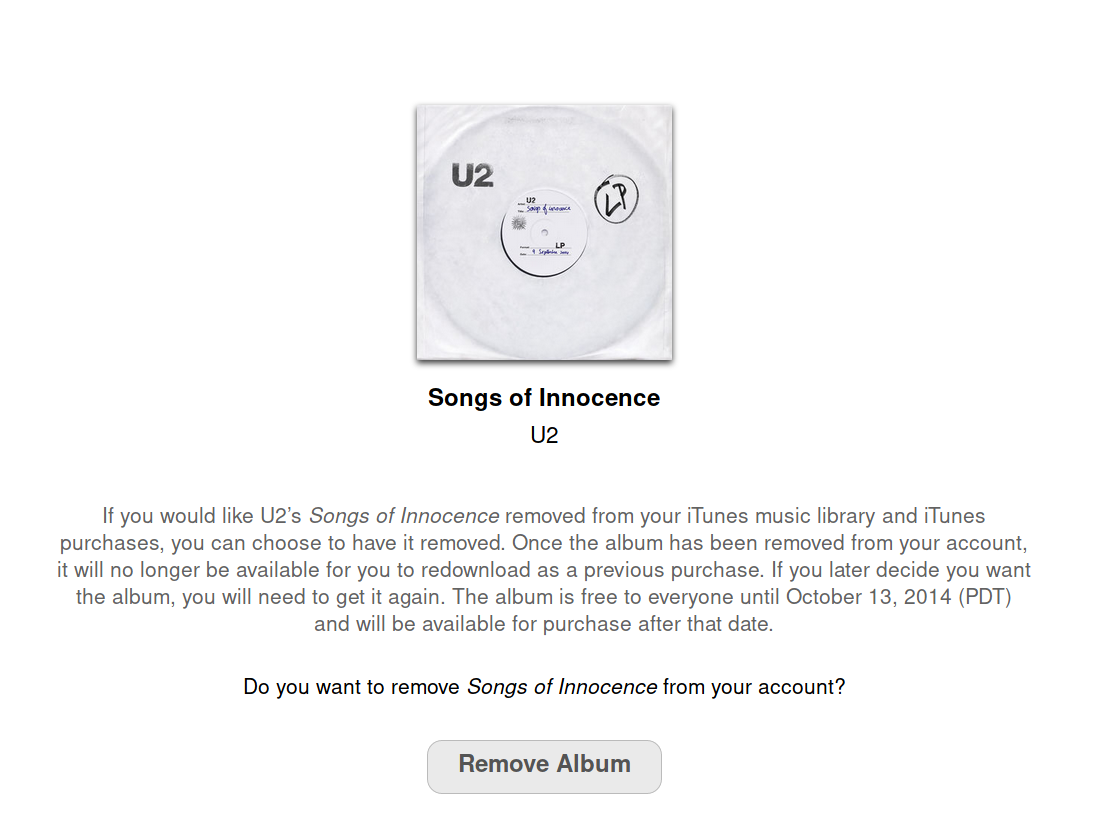
\includegraphics[height=7cm]{images/u2.png}
\end{center}
\end{onlyenv}
\end{frame}

\begin{frame}[label={sec:org646d460},fragile]{Rolling out U2}
 \begin{minted}[]{haskell}
type U2 a = U (U a)
\end{minted}
\end{frame}

\begin{frame}[label={sec:org77433b0},fragile]{Moving around in the \sout{complex} Universe}
 \begin{minted}[]{haskell}
shift :: Direction -> U2 a -> U2 a
shift North u = left      u
shift South u = right     u
shift East  u = right <$> u
shift West  u = left  <$> u
\end{minted}

\begin{columns}
\begin{column}{0.45\columnwidth}
\begin{onlyenv}<2->
\begin{minted}[,escapeinside=||,mathescape=true]{haskell}
> print' DisplayFocused . narrow2 3 $ gol1
|$\ \square\square\square[\square]\square\square\square$|
|$\ \square\square\square[\square]\square\square\square$|
|$\ \square\square\square[\square]\square\square\square$|
|$[\square\square\square\ \square\ \square\square\square]$|
|$\ \square\square\square[\square]\blacksquare\blacksquare\blacksquare$|
|$\ \square\square\square[\square]\blacksquare\blacksquare\square$|
|$\ \square\square\square[\square]\blacksquare\blacksquare\square$|
\end{minted}
\end{onlyenv}
\end{column}

\begin{column}{0.45\columnwidth}
\begin{onlyenv}<3>
\begin{minted}[,escapeinside=||,mathescape=true]{haskell}
> (...) . shift North $ gol1
|$\ \square\square\square[\square]\square\square\square$|
|$\ \square\square\square[\square]\square\square\square$|
|$\ \square\square\square[\square]\square\square\square$|
|$[\square\square\square\ \square\ \square\square\square]$|
|$\ \square\square\square[\square]\square\square\square$|
|$\ \square\square\square[\square]\blacksquare\blacksquare\blacksquare$|
|$\ \square\square\square[\square]\blacksquare\blacksquare\square$|
\end{minted}
\end{onlyenv}

\begin{onlyenv}<4>
\begin{minted}[,escapeinside=||,mathescape=true]{haskell}
> (...) . shiftn 3 South . shiftn 3 East $ gol1
|$\ \square\square\square[\square]\square\square\square$|
|$\ \square\blacksquare\blacksquare[\blacksquare]\blacksquare\blacksquare\square$|
|$\ \square\blacksquare\blacksquare[\square]\blacksquare\blacksquare\square$|
|$[\square\blacksquare\blacksquare\ \square\ \blacksquare\blacksquare\square]$|
|$\ \square\blacksquare\blacksquare[\square]\blacksquare\blacksquare\square$|
|$\ \square\blacksquare\blacksquare[\blacksquare]\blacksquare\blacksquare\square$|
|$\ \square\square\square[\square]\square\square\square$|
\end{minted}
\end{onlyenv}
\end{column}
\end{columns}
\end{frame}

\begin{frame}[label={sec:orge68b430},fragile]{Game of Life rules}
 \begin{minted}[]{haskell}
rule :: U (U Cell) -> Cell
rule u | ns == 3   = Alive
       | ns == 2   = extract . extract $ u
       | otherwise = Dead
  where ns = length . filter (== Alive) . neighbours Dead $ u

--------------------------------------------------------------------------------

neighbours :: Cell -> U (U Cell) -> [Cell]
neighbours c u
  = fmap (\f -> extract . extract $ f u)
    [ shift North
    , shift North . shift East
    , shift East
    , shift East . shift South
    , shift South
    , shift South . shift West
    , shift West
    , shift West . shift North
    ]
\end{minted}
\end{frame}

\begin{frame}[label={sec:org78df5fa},fragile]{Was easy, right?}
 \begin{minted}[]{haskell}
> let someGol = undefined :: U (U Cell)
\end{minted}

\pause

\begin{minted}[]{haskell}
> :t rule someGol
rule someGol :: Cell
\end{minted}

\pause

\begin{minted}[]{haskell}
> :t extend rule someGol
extend rule someGol :: U Cell
\end{minted}

\pause

Wait\ldots{} WAT?
\end{frame}

\begin{frame}[label={sec:org1bd4736},fragile]{Extending 2D Universe (1)}
 \begin{minted}[]{haskell}
> :t extend
extend :: (U a -> b) -> U a -> U b
\end{minted}

\pause

\begin{minted}[]{haskell}
> :t extend rule
extend rule' :: U (U Cell) -> U Cell
\end{minted}

\pause

But we need \texttt{extend2 :: (U (U a) -> b) - U (U a) -> U (U b)}.
\end{frame}

\begin{frame}[label={sec:org7a1c1b8},fragile]{Extending 2D Universe (2)}
 \begin{minted}[]{haskell}
duplicate2 :: U (U a) -> U (U (U (U a)))
duplicate2 = fmap duplicate . duplicate

extend2 :: (U (U a) -> b) -> U (U a) -> U (U b)
extend2 f = fmap (fmap f) . duplicate2
\end{minted}

\pause

\begin{equation*}
  \begingroup
  \setlength\arraycolsep{0.25pt}
  \renewcommand{\arraystretch}{0.5}
  \begin{matrix}
    \square & \square & \square      & \square      & \square \\
    \square & \square & \blacksquare & \square      & \square \\
    \square & \square & \blacksquare & \square      & \square \\
    \square & \square & \blacksquare & \square      & \square \\
    \square & \square & \square      & \square      & \square \\
  \end{matrix}\Rightarrow
  \begin{matrix}
    \square & \square & \square & \square & \square \\
    \square & \square & \square & \square & \square \\
    \square & \square & \square & \square & \square \\
    \square & \square & \square & \square & \square \\
    \square & \square & \square & \square & \square \\
  \end{matrix}\ne
  \begin{matrix}
    \square & \square      & \square      & \square      & \square \\
    \square & \square      & \square      & \square      & \square \\
    \square & \blacksquare & \blacksquare & \blacksquare & \square \\
    \square & \square      & \square      & \square      & \square \\
    \square & \square      & \square      & \square      & \square \\
  \end{matrix}
  \endgroup
\end{equation*}

\pause

fmap-fu can't always save you, functor-kun!
\end{frame}

\begin{frame}[label={sec:org6301367},fragile]{Actually extending 2D Universe}
 \begin{minted}[]{haskell}
newtype U2 a
  = U2
  { getUniverse :: U (U a)
  } deriving (Functor)

extract :: U2 a -> a
extract = extract . extract . getUniverse

duplicate :: U2 a -> U2 (U2 a)
duplicate = fmap U2 . U2 . shifted . shifted . getUniverse
  where shifted :: U (U a) -> U (U (U a))
        shifted u@(U _ (U ls _ rs) _) = U
          (tail $ iterate (fmap left) u)
          u
          (tail $ iterate (fmap right) u)

extend :: (U2 a -> a) -> U2 a -> U2 a
extend f = fmap f . duplicate
\end{minted}
\end{frame}

\begin{frame}[label={sec:org248ac5c},fragile]{Works}
 \begin{minted}[,escapeinside=||,mathescape=true]{haskell}
> mapM_ (print . narrow2' 0 4 0 4) . take 2 . iterate (extend rule) $ gol3
|$\square\square\square\square\square$|
|$\square\square\blacksquare\square\square$|
|$\square\square\blacksquare\square\square$|
|$\square\square\blacksquare\square\square$|
|$\square\square\square\square\square$|
|$$|
|$\square\square\square\square\square$|
|$\square\square\square\square\square$|
|$\square\blacksquare\blacksquare\blacksquare\square$|
|$\square\square\square\square\square$|
|$\square\square\square\square\square$|
\end{minted}
\end{frame}

\begin{frame}[label={sec:orgcbc1484}]{(not so) Final words}
\begin{itemize}
\item <1-> Moving from 1D to 2D is really simple (not counting the wasted time on the
wrong idea).
\item <2-> Great abstraction for our task.
\item <3-> It's easy to implement other automata on top of this abstraction.
\begin{itemize}
\item Different cells (more values)
\item Different rules (more neighbours)
\end{itemize}
\end{itemize}
\end{frame}

\section{Act 3: Bomberman}
\label{sec:orga69ea93}

\begin{frame}[label={sec:org32bc293}]{Definition}
\pause

Do you really need a definition of Bomberman?
\end{frame}

\begin{frame}[label={sec:orgf88673b}]{Definition}
\begin{center}
\includegraphics[width=.9\linewidth]{images/bomberman-1.jpg}
\end{center}
\end{frame}

\begin{frame}[label={sec:orgd254cf5}]{But we have a different one}
\begin{center}
\includegraphics[height=8cm]{images/bomberman-2.png}
\end{center}
\end{frame}

\begin{frame}[label={sec:org297f035}]{Bells and whistles}
\begin{center}
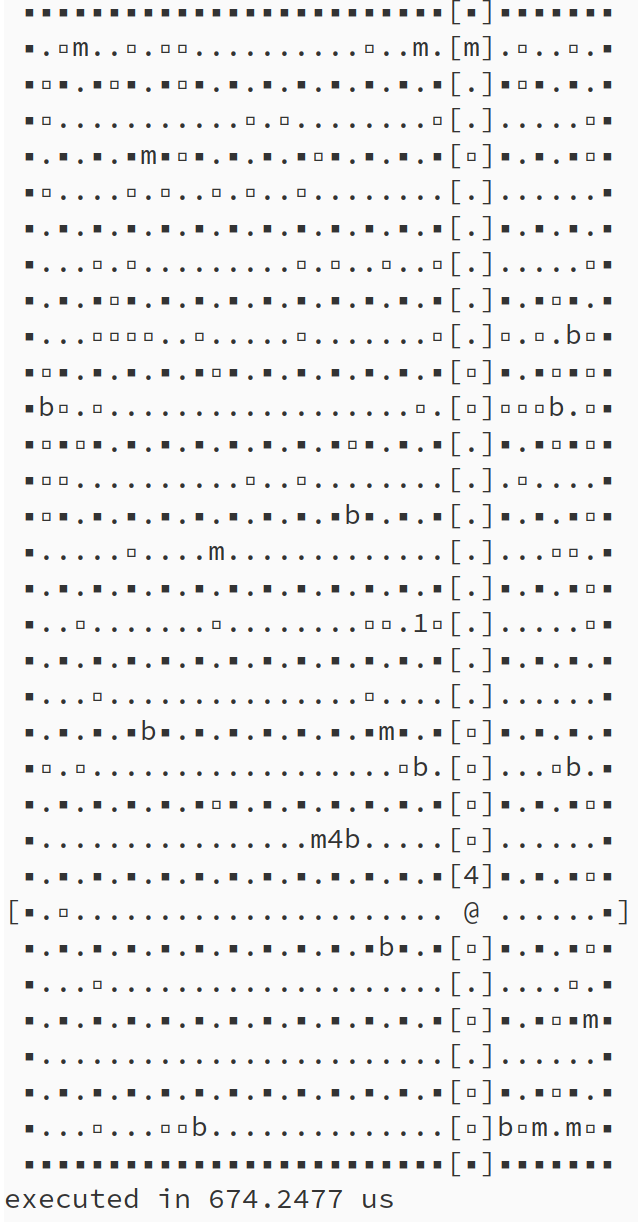
\includegraphics[height=8cm]{images/bomberman-3.png}
\end{center}
\end{frame}

\begin{frame}[label={sec:org9cdd8f2},fragile]{Reusing U2}
 \begin{minted}[]{haskell}
data Cell
  = Bomberman
  | BombBomberman
  | DeadBomberman

  | OtherBomberman
  | OtherBombBomberman
  | OtherDeadBomberman

  | BombTimer5
  | BombTimer4
  | BombTimer3
  | BombTimer2
  | BombTimer1
  | Boom

  | Wall
  | DestroyableWall
  | DestroyedWall

  | MeatChopper
  | DeadMeatChopper

  | Empty
\end{minted}
\end{frame}

\begin{frame}[label={sec:org18f70f9},fragile]{What is bot?}
 \begin{minted}[]{haskell}
bot :: ( MonadIO m
       , MonadReader r m
       , HasLogFunc r
       )
    => U2 Cell
    -> m Action
bot = undefined
\end{minted}

\pause

What to \texttt{extend}?
\end{frame}

\begin{frame}[label={sec:orgbfca5d8}]{What we care about}
\begin{itemize}
\item <1-> Greed. What can be destroyed?
\item <2-> Safety. What can kill us?
\end{itemize}
\end{frame}

\begin{frame}[label={sec:org75926d6},fragile]{Fatum of the Universe}
 \begin{minted}[]{haskell}
data MarkedCell
  = MarkedCell
  { getCell        :: !Cell
  , getDangers     :: ![Cell]
  , getTargets     :: ![Cell]
  }
\end{minted}

\pause

\begin{minted}[]{haskell}
mark :: U2 Cell -> MarkedCell
mark board = MarkedCell (extract board) dangers targets
  where dangers = bombs <> monsters
        bombs = filter isBomb (allVisible (not . isAnyWall) 3 board)
        monsters = filter (isMonster .| isEnemy) (allVisible (not . isAnyWall) 1 board)

        targets
          = filter (isDestroyableWall .| isMonster .| isEnemy)
          $ allVisible (not . isWall) 3 board
\end{minted}
\end{frame}

\begin{frame}[label={sec:org77ad16a},fragile]{Fatum of the Universe}
 \begin{minted}[]{haskell}
> :t extend
extend :: (U2 a -> b) -> U2 a -> U2 b

> :t extend mark
extend mark :: U2 Cell -> U2 MarkedCell
\end{minted}
\end{frame}

\begin{frame}[label={sec:org0f53a17},fragile,t]{The bot}
 \begin{onlyenv}<1>
\begin{minted}[]{haskell}
bot :: ( MonadIO m
       , MonadReader r m
       , HasLogFunc r
       )
    => U2 Cell
    -> m Action
bot board = do
  let markedBoard = extend mark $ narrow 11 board
  ...
\end{minted}
\end{onlyenv}

\begin{onlyenv}<2>
\begin{minted}[]{haskell}
bot :: ( MonadIO m
       , MonadReader r m
       , HasLogFunc r
       )
    => U2 Cell
    -> m Action
bot board = do
  let markedBoard = extend mark $ narrow 11 board
      directions  = if isSafe . extract $ markedBoard
                    then ...
                    else ...
  ...

isSafe :: MarkedCell -> Bool
isSafe = L.null . getDangers
\end{minted}
\end{onlyenv}

\begin{onlyenv}<3>
\begin{minted}[]{haskell}
bot :: ( MonadIO m
       , MonadReader r m
       , HasLogFunc r
       )
    => U2 Cell
    -> m Action
bot board = do
  let markedBoard = extend mark $ narrow 11 board
      directions  = if isSafe . extract $ markedBoard
                    then directionsToTargets markedBoard
                    else escapeDirections markedBoard
  ...

isSafe :: MarkedCell -> Bool
isSafe = L.null . getDangers
\end{minted}
\end{onlyenv}

\begin{onlyenv}<4>
\begin{minted}[]{haskell}
bot :: ( MonadIO m
       , MonadReader r m
       , HasLogFunc r
       )
    => U2 Cell
    -> m Action
bot board = do
  let markedBoard = extend mark $ narrow 11 board
      directions  = if isSafe . extract $ markedBoard
                    then directionsToTargets markedBoard
                    else escapeDirections markedBoard
  direction <- randomElement directions
  ...

isSafe :: MarkedCell -> Bool
isSafe = L.null . getDangers
\end{minted}
\end{onlyenv}

\begin{onlyenv}<5>
\begin{minted}[]{haskell}
bot :: ( MonadIO m
       , MonadReader r m
       , HasLogFunc r
       )
    => U2 Cell
    -> m Action
bot board = do
  let markedBoard = extend mark $ narrow 11 board
      directions  = if isSafe . extract $ markedBoard
                    then directionsToTargets markedBoard
                    else escapeDirections markedBoard
  direction <- randomElement directions
  let bomb = shouldBomb markedBoard direction
  ...

isSafe :: MarkedCell -> Bool
isSafe = L.null . getDangers
\end{minted}
\end{onlyenv}

\begin{onlyenv}<6>
\begin{minted}[]{haskell}
bot :: ( MonadIO m
       , MonadReader r m
       , HasLogFunc r
       )
    => U2 Cell
    -> m Action
bot board = do
  let markedBoard = extend mark $ narrow 11 board
      directions  = if isSafe . extract $ markedBoard
                    then directionsToTargets markedBoard
                    else escapeDirections markedBoard
  direction <- randomElement directions
  let bomb = shouldBomb markedBoard direction
  pure $ maybe (Action Stay bomb) (flip Action bomb . Move) direction

isSafe :: MarkedCell -> Bool
isSafe = L.null . getDangers
\end{minted}
\end{onlyenv}
\end{frame}

\begin{frame}[label={sec:org593aab4}]{Danger! Live demo}
\emph{Live demos are subject to fail. Accept and forgive. Move on.}
\end{frame}

\begin{frame}[label={sec:org14e79d5}]{(not so) Final words}
\begin{itemize}
\item <1-> Great abstraction for our task. Again.
\begin{itemize}
\item We care about elements surrounding player.
\item Easy to mark all the interesting points to be used in our bot logic.
\end{itemize}
\item <2-> Not all topics are covered.
\begin{itemize}
\item Path finding. Data type helps us here.
\item Being a smart bot.
\end{itemize}
\item <3-> Now you understand the last bit of the title.
\item <4-> Do you think we are done?
\end{itemize}
\end{frame}

\section{Finale}
\label{sec:org9aeebd1}

\begin{frame}[label={sec:org4e0e7a5},fragile]{Commonalities (1)}
 \begin{minted}[]{haskell}
extract :: U a  -> a
extract :: U2 a -> a
\end{minted}

\pause

\begin{minted}[]{haskell}
extract :: f a -> a
\end{minted}
\end{frame}

\begin{frame}[label={sec:org53510bd},fragile]{Commonalities (2)}
 \begin{minted}[]{haskell}
extend :: (U a -> b) -> U a  -> U a
extend :: (U2 a -> b) -> U2 a -> U2 b
\end{minted}

\pause

\begin{minted}[]{haskell}
extend :: (f a -> b) -> f a -> f b
\end{minted}
\end{frame}

\begin{frame}[label={sec:org4728c94},fragile]{Comonad}
 \begin{minted}[]{haskell}
class Functor f => Comonad f where
  extract :: f a -> a
  extend :: (f a -> b) -> f a -> f b
  duplicate :: f a -> f (f a)
\end{minted}

\pause

\texttt{Comonad} laws:

\begin{minted}[]{haskell}
extend extract      = id
extract . extend f  = f
extend f . extend g = extend (f . extend g)
\end{minted}
\end{frame}

\begin{frame}[label={sec:orgc8528af},fragile]{Co-monad}
 \begin{columns}
\begin{column}{0.45\columnwidth}
\begin{minted}[]{haskell}
extract :: f a -> a
(=>>) :: f a -> (f a -> b) -> f b
\end{minted}
\end{column}

\begin{column}{0.45\columnwidth}
\begin{minted}[]{haskell}
return :: a -> f a
(>>=) :: f a -> (a -> f b) -> f b
\end{minted}
\end{column}
\end{columns}
\end{frame}

\begin{frame}[label={sec:org76ed1c7},fragile]{Universe is Comonad}
 That should be obvious by now.

\pause

\begin{minted}[]{haskell}
instance Comonad U where
  extract (U _ x _) = x
  duplicate u = U (tail $ iterate left u) u (tail $ iterate right u)

instance Comonad U2 where
  extract = extract . extract . getUniverse
  duplicate = fmap U2 . U2 . shifted . shifted . getUniverse
    where shifted :: U (U a) -> U (U (U a))
          shifted u@(U _ (U ls _ rs) _) = U
            (tail $ iterate (fmap left) u)
            u
            (tail $ iterate (fmap right) u)
\end{minted}
\end{frame}

\begin{frame}[label={sec:org7920569},fragile]{Store}
 \begin{minted}[]{haskell}
data Store s a = Store (s -> a) s

extract (Store f s) = f s

duplicate (Store f s) = Store (Store f) s
\end{minted}

\pause

\emph{Homework:} solve ECA and GoL using \texttt{Store} data type.
\end{frame}

\begin{frame}[label={sec:org53b3dd3}]{Many uses}
\begin{itemize}
\item <1-> Instances
\begin{itemize}
\item Pointed lists (Universe)
\item Functions returning monoids.
\item Store
\end{itemize}
\item <2-> Problems
\begin{itemize}
\item Cellular automata.
\item Discrete board games.
\item Window manager (XMonad).
\item Builder patter.
\item Iterator pattern.
\item Command pattern.
\item FRP.
\end{itemize}
\end{itemize}
\end{frame}

\begin{frame}[label={sec:org5829a9d}]{Final words}
\begin{itemize}
\item <1-> Comonads give us an interface for extracting and extending certain data
types.
\item <2-> They also provide a 'method' like notation to Haskell.
\item <3-> Comonads are flipped Monads.
\item <4-> Using this interface we solved 3 different problems.
\end{itemize}
\end{frame}

\begin{frame}[label={sec:org5e860fe}]{Grab the code}
\url{https://github.com/d12frosted/talks}
\end{frame}

\section*{References}
\label{sec:orged78944}
\begin{frame}[label={sec:orgca59229}]{References}
\begin{itemize}
\item \url{https://www.st.cs.uni-saarland.de/edu/seminare/2005/advanced-fp/docs/huet-zipper.pdf}
\item \url{http://mathworld.wolfram.com/CellularAutomaton.html}
\item \url{http://mathworld.wolfram.com/ElementaryCellularAutomaton.html}
\item \url{http://mathworld.wolfram.com/GameofLife.html}
\item \url{https://hackage.haskell.org/package/comonad}
\item \url{https://bartoszmilewski.com/2017/01/02/comonads/}
\item \url{http://blog.sigfpe.com/2006/12/evaluating-cellular-automata-is.html}
\item \url{http://www.haskellforall.com/2013/02/you-could-have-invented-comonads.html}
\end{itemize}
\end{frame}

\section{Questions?}
\label{sec:org963d632}
\section{Thank you}
\label{sec:org0ecad66}
\end{document}
